%-----------------------------------------------------------------------
%;  Copyright (C) 2006
%;  Associated Universities, Inc. Washington DC, USA.
%;
%;  This program is free software; you can redistribute it and/or
%;  modify it under the terms of the GNU General Public License as
%;  published by the Free Software Foundation; either version 2 of
%;  the License, or (at your option) any later version.
%;
%;  This program is distributed in the hope that it will be useful,
%;  but WITHOUT ANY WARRANTY; without even the implied warranty of
%;  MERCHANTABILITY or FITNESS FOR A PARTICULAR PURPOSE.  See the
%;  GNU General Public License for more details.
%;
%;  You should have received a copy of the GNU General Public
%;  License along with this program; if not, write to the Free
%;  Software Foundation, Inc., 675 Massachusetts Ave, Cambridge,
%;  MA 02139, USA.
%;
%;  Correspondence concerning AIPS should be addressed as follows:
%;          Internet email: aipsmail@nrao.edu.
%;          Postal address: AIPS Project Office
%;                          National Radio Astronomy Observatory
%;                          520 Edgemont Road
%;                          Charlottesville, VA 22903-2475 USA
%-----------------------------------------------------------------------
%Body of intermediate AIPSletter for 31 December 2006

\documentclass[twoside]{article}
\usepackage{graphics}

\newcommand{\AIPRELEASE}{June 30, 2006}
\newcommand{\AIPVOLUME}{Volume XXVI}
\newcommand{\AIPNUMBER}{Number 1}
\newcommand{\RELEASENAME}{{\tt 31DEC06}}
\newcommand{\NEWNAME}{{\tt 31DEC06}}
\newcommand{\OLDNAME}{{\tt 31DEC05}}

%macros and title page format for the \AIPS\ letter.
\input LET98.MAC
%\input psfig

\newcommand{\MYSpace}{-11pt}

\normalstyle

\section{General developments in \AIPS}

\subsection{Current and future releases}

We now have formal \AIPS\ releases on an annual basis.  Beginning near
the end of 2004, we have made available full binary installation
methods for both the frozen and development versions for MacIntosh
OS/X (PPC), Solaris, and Linux.  A binary release of {\tt 31DEC06} is
now available for MacIntosh OS/X with the Intel cpu chip.  All
architectures can do a full installation from the source files.  The
next release is called \RELEASENAME\ and remains under active
development.  You may fetch and install a copy of this version at any
time using {\it anonymous} {\tt ftp} for source-only copies and {\tt
rsync} for binary copies.  This \Aipsletter\ is intended to advise you
of developments to date in this new release. Having fetched
\RELEASENAME, you may update your installation whenever you want by
running the so-called ``Midnight Job'' (MNJ) which uses transaction
files to copy and compile the code selectively based on the code
changes and compilations we have done.  The MNJ will also update sites
that have done a binary installation using {\tt rsync}.  There is a
guide to the install script and an \AIPS\ Manager FAQ page on the
\AIPS\ web site.

The MNJ serves up \AIPS\ incrementally using the Unix tool {\tt cvs}
running with anonymous ftp.  The binary MNJ also uses the tool {\tt
rsync} as does the binary installation.  Linux sites will almost
certainly have {\tt cvs} installed; other sites may have installed it
along with other GNU tools.  Secondary MNJs will still be possible
using {\tt ssh} or {\tt rcp} or NFS as with previous releases.  We
have found that {\tt cvs} works very well, although it has one quirk.
If a site modifies a file locally but in an \AIPS-standard directory,
{\tt cvs} will detect the modification and attempt to reconcile the
local version with the NRAO-supplied version.  This usually produces a
file that will not compile or run as intended.

\AIPS\ is now copyright \copyright\ 1995 through 2006 by Associated
Universities, Inc., NRAO's parent corporation, but may be made freely
available under the terms of the Free Software Foundation's General
Public License (GPL)\@.  This means that User Agreements are no longer
required, that \AIPS\ may be obtained via anonymous ftp without
contacting NRAO, and that the software may be redistributed (and/or
modified), under certain conditions.  The full text of the GPL can be
found in the \texttt{15JUL95} \Aipsletter, in each copy of \AIPS\
releases, and on the web at {\tt
  http://www.aoc.nrao.edu/aips/COPYING}.
\vfill\eject

\section{Patch Distribution for \OLDNAME}

Important bug fixes and selected improvements in \OLDNAME\ can be
downloaded via the Web beginning at:

\begin{center}
\vskip -10pt
{\tt http://www.aoc.nrao.edu/aips/patch.html}
\vskip -10pt
\end{center}

Alternatively one can use {\it anonymous} \ftp\ to the NRAO server
{\tt ftp.aoc.nrao.edu}.  Documentation about patches to a release is
placed on this site at {\tt pub/software/aips/}{\it release-name} and
the code is placed in suitable subdirectories below this.  As bugs in
\NEWNAME\ are found, they are simply corrected since \NEWNAME\ remains
under development.  Corrections and additions are made with a midnight
job rather than with manual patches.
The patch system has changed because we now have binary installations.
We now actually patch the master version of \OLDNAME, which means that
a MNJ run on \OLDNAME\ after the patch will fetch the corrected code
and/or binaries rather than failing.  Also, installations of \OLDNAME\
after the patch date will contain the corrected code.

The \OLDNAME\ release had a few important patches most of which were
released in April when we changed the patch system.  All changes were
made on 2006-02-21 and are
\begin{enumerate}
\item\ {\tt DBCON} did not handle differences in frequency increment
      between {\tt FQ} entries properly when changing reference
      channel to 1
\item\ {\tt DSMEAR} subroutine did not handle {\tt FQ} ID 0 correctly,
      affecting VLBI data with significant delays
\item\ {\tt SAD}  had an error in round off for RA and Dec display
\item\ {\tt WIPER} did not handle source ID numbers correctly causing
      elevation et al.~to be incorrect on single-source files
\item\ {\tt SETFC} had a mathematical error in setting the X coordinate
      of boxes around NVSS sources
\item\ {\tt INTERPLATE} subroutines assigned a {\tt LONGINT} to an
      {\tt INTEGER} causing trouble on AMD-64s
\end{enumerate}

\section{Improvements of interest in \RELEASENAME}

We expect to continue publishing the  \Aipsletter\ approximately every
six months along with the annual releases.  There have been quite a
few changes in \RELEASENAME\ in the last six months.  Many have been
the usual bug fixes, but there have also been a number of new verbs,
tasks, and procedures as well as significant improvements in existing
tasks.  New tasks include {\tt ANBPL} which plots and prints \uv\
data, particularly weights, converted to antenna-based values, {\tt
UVHIM} which constructs images of two-dimensional histograms of \uv\
data, and {\tt DDBGR} which displays the contents of disk files for
debugging purposes.  New verbs include {\tt PLGET} which sets a task's
adverbs to those used when making a selected plot file, {\tt DELBOX}
which deletes Clean boxes in {\tt CLBOX} interactively, {\tt DFILEBOX}
which deletes Clean boxes in a {\tt BOXFILE} interactively, and {\tt
GETPOPSN} which returns the \POPS\ number of the {\tt AIPS} session
for use in procedures.  New {\tt RUN} file procedures include {\tt
STUFFR} which merges multiple days worth of \uv\ data into a much more
compact data set and {\tt PEELR} which performs a nearly magical
self-calibration of image facets containing ``interfering'' sources.
\AIPS\ support for MacIntosh OS/X systems using Intel cpu chips has
been implemented including binary installations based on the Intel
compiler.

{\tt 31DEC04} through \RELEASENAME\ use a new numbering scheme for
magnetic tape logical unit numbers that is incompatible with previous
versions.  Thus all tape tasks and the server {\tt TPMON} must be from
one of these three releases.  Other than this, \RELEASENAME\ is
compatible in all major ways with the with the {\tt 15OCT98} and later
releases.  There are significant incompatibilities with older versions.

\subsection{UV data calibration and handling}

\subsubsection{Amplitude Calibrator Models for the VLA}

It is well known that the main amplitude calibrators for the VLA are
resolved at most frequencies and configurations.  Where they are not
heavily resolved (\eg\ L-band D-array), there are confusing sources.
The best way to determine the amplitude calibration of the VLA
antennas directly is to use detailed models of the source structure of
these calibrators.  See as an example the first of the color pages at
the end of this \Aipsletter\ which shows an image and \uv\ plot of
3C48 at X band.

In the {\tt 30JUN04} edition of the \Aipsletter\ we announced the
availability in \AIPS\ of VLA flux calibrator models for the 3 highest
frequency bands observed with the VLA\@.  Here we announce the
availability of flux calibrator models for all bands from K through L
of 3C48 and 3C286, all bands K through C for 3C138, in addition to the
models for K, Q and U for 3C147\@.  Additional models for 3C138 and
3C147 at the lower frequencies will become available over the next
year.  To see what models are available in \AIPS\ type {\tt CALDIR};
to load a model use the task {\tt CALRD}\@.  The models shipped with
\AIPS\ are postage stamps of the central source and all Clean
Components.  The full model images and components are available for
download from {\tt http://www.aoc.nrao.edu/$\sim$cchandle/cal/cal.html} (Q,
K and U-bands) and {\tt http://www.aoc.nrao.edu/$\sim$amiodusz/vlacal.html}
(X, C and L-bands)

Now that most VLA primary flux calibrators have models, their use
should be the default when calibrating amplitudes on the VLA.  See the
updated Chapter 4 of the\AIPS\ \Cookbook\ for details on this.  As
mentioned above, the VLA primary flux calibrators are resolved at most
frequencies and configurations.  Even in the configurations and
frequencies where they are not resolved there are many confusing
sources, so in {\it all situations} a model will make the flux
calibration more accurate. When models are used, there is no need to
limit the \uv\ range or antennas when running {\tt CALIB}, which in
turn will make automated data reduction easier.  For example, the
\AIPS\ pipeline procedure {\tt VLARUN} automatically uses the models
if they exist.

\subsubsection{{\tt ANBPL}}

{\tt ANBPL} or ``antenna-based plot'' is a new task to print and plot
antenna-based quantities determined from baseline-based visibilities.
weights, amplitudes, phases, reals, and imaginaries computed in a
couple of ways can be plotted against time, elevation, hour angle,
azimuth, and parallactic angle.  The plots are similar to ones from
{\tt VPLOT} and the printed outputs are in the {\tt LIST} form of {\tt
LISTR} more or less with user control of the number of digits.  Plots
of weight against time have been found to be a very good diagnostic of
difficulties in calibration and self-calibration.  In fact, a user
commented that ``it is scary to think how long we have used the VLA
without this task.''

\subsubsection{{\tt VLARUN}}

Lorant Sjouwerman has developed a pipeline to edit, calibrate, and
image VLA data.  A preliminary version of this pipeline has been
available in \AIPS\ for several years, but a new, more complete
version was released in March.  The {\tt RUN} file {\tt VLARUN}
compiles a number of procedures including the main user-level
procedure also named {\tt VLARUN}\@.  The pipeline begins by doing
some automatic flagging using {\tt QUACK} and {\tt FLAGR} in its {\tt
  TIME} mode. Then it runs {\tt SETJY} to clear the source table and
calculate fluxes for standard calibrators or set user-specified
fluxes.  Then {\tt CALIB} is run for phases using calibrator models
where available and the {\tt CL} table updated with {\tt CLCAL}\@.
{\tt CALIB} is then run for amplitudes on phase-calibrated data using
models where available, {\tt GETJY} determines the secondary
calibrator fluxes, and {\tt CLCAL} again updates the {\tt CL} table.
For line data, tables are copied to the spectral-line \uv\ file and
{\tt BPASS} is run to determine a bandpass function.  In the imaging
phase, the data are {\tt SPLIT}, imaging parameters are determined
with {\tt SETFC} including if needed multi-facet {\tt BOXFILE}s, and
then {\tt IMAGR} run to make images of all sources in the data set.
If requested, {\tt SCIMG} is used instead of {\tt IMAGR} to do several
cycles of imaging with self-calibration.

There seems to be a widespread distrust of pipeline data reductions.
Nonetheless, these systems are capable of producing quite good results
in favorable cases.  In fact, it usually fails only when there are
serious problems with the data such as bad atmosphere or ionosphere,
absorption lines in the bandpass calibrators, and the like.  A number
of images produced by {\tt VLARUN} with no hand massaging are
reproduced on the second color page at the end of the \Aipsletter.  At
present, {\tt VLARUN} has quite a number of adverbs to allow the user
to limit what the procedure attempts to do. It produces a large number
of plots which the user may view to determine if the results look
reasonable.  Future developments in this pipeline will include tools
to examine the calibration tables for the user and tools to calibrate
and image polarization when appropriate. Pipelines are intended to
produce a ``standard product'' of calibrated data and images for
archiving with little or no human intervention.  As such, they are not
expected to allow truly interactive operations including hand editing
of \uv\ data, hand setting of Clean boxes, and the like.  Nonetheless,
it should not be too hard to offer a version with more extensive
interactivity that could allow these and other interactions for users
processing their own data.  When used by the observer, {\tt VLARUN}
may be executed once simply to identify bad data and then re-executed
after manual editing.  This should yield a nicely calibrated data set
to start self-calibration.

\subsubsection{{\tt VBGLU} and {\tt VBMRG}}

The VLBA correlator is in the process of being converted entirely to
Mark 5 (disk-based) playback.  The number of playback units is still
limited and so it may be necessary for multiple passes through the
correlator in order to correlate all antennas with all other antennas.
Inevitably, many baselines will be repeated between these passes.
Users in this situation, should load all of their data to disk with
{\tt FITLD}\@.  The multiple passes must be concatenated, which can be
done by {\tt FITLD} or, after loading into separate files, by {\tt
DBCON}\@.  The old task {\tt VBMRG} has been resurrected and
modernized in {\tt 31DEC06} to strip out duplicate correlations from
such data sets after they have been sorted into {\tt BT} order by {\tt
UVSRT}\@.

The bandwidth of the VLBA correlator is also limited.  In order to
achieve wider bandwidth, different frequencies may be correlated in
separate passes through the correlator.  These frequencies may be put
into a full bandwidth data set with {\tt VBGLU}\@.  In {\tt 31DEC06},
{\tt VBGLU} was re-written with more efficient algorithms which
recover all of the input data even if the input data sets are not
identical.  Previously, only those times present in the first input
data set appeared in the output data sets and there were significant
errors when the later data sets had more than a few times not
appearing in the first data set.

\subsubsection{{\tt STUFFR}}

Deep integrations on chosen fields are currently very popular in
astronomy.  Radio observations of this type usually involve multiple
days on the same pointing position with the same array configuration.
After doing an initial round of editing, calibration, and
self-calibration on each day individually, it is normal to want to
combine all days' data in order to do the final imaging.  For
efficiency, these enormous data sets need to be compressed in some
way.  The new {\tt RUN} file named {\tt STUFFR} compiles a procedure
of the same name to perform this operation.  The procedure loops
through the input files changing the times to hour angles with {\tt
TI2HA}, sorting into {\tt BT} order, altering the observation date,
and concatenating with {\tt DBCON}\@.  The final full data set is then
time averaged using a baseline-dependent integration time with {\tt
UBAVG} and is finally sorted back into {\tt TB} order with {\tt
UVSRT}\@.  Like {\tt PEELR} described below, this procedure only
implements things that have been available in \AIPS\ for some time.
However, it does it efficiently, deleting all temporary files as soon
as they are no longer needed, and it does it without the errors that
are so easy to make when one attempts a complicated sequence by hand.

\subsubsection{Other \uv-editing matters}

\begin{description}
\myitem{UVFLG} was changed so that the {\tt UFLG} operation uses all
           adverbs including {\tt REASON} in a very general way,
           making the {\tt REAS} option meaningless.
\myitem{FLAGR} was overhauled to perform its operation on up to four
           polarizations as selected by the user.  Apparently, RFI is
           sometimes much more visible on the cross-hand
           polarizations.
\myitem{WIPER} was changed to plot axis labels when possible in its
           display.  It was revised to allow simultaneous editing of
           both parallel-hand polarizations.  History-file writing was
           added and an error causing it to fail to find elevations
           and the like for single-source files was corrected.
\myitem{EDITR} and {\tt EDITA} were changed to offer the choice of
           flagging the current source or all sources.  Corrected
           error that caused it to fail to find the nearest point when
           the user pointed exactly at it.
\myitem{TVFLG} was revised to offer the options to {\tt LOAD NEXT
           CHAN} and {\tt LOAD PREV CHAN} to speed editing of a
           multi-channel data set.
\myitem{SNEDT} was changed to allow editing {\tt TY} tables as
           calibration tables.  A {\tt SET VALUES} function was added
           for both table types and a number of problems affecting
           ``crowded'' displays in particular were corrected.
\end{description}

\subsubsection{Other \uv-display matters}

\begin{description}
\myitem{UVHGM} was overhauled to support the full range of calibration
         adverbs and more {\tt STOKES} values and to offer the option
         to fit the histograms with Gaussians.
\myitem{UVHIM} is a new task to compute a two-dimensional histogram of
         a \uv\ data set.  It write this out as a standard image
         making all image display functions available.  The two axes
         of the image are chosen from visibility real, imaginary,
         amplitude, phase, and weight, time, and baseline $u, v, w$,
         length, and position angle.  For example, an image of
         visibility real versus imaginary will illustrate the amplitude
         and phase stability (or lack thereof)
\myitem{BPLOT} was given a {\tt PDIF} option to difference phase with
         average phase rather than doing vector differences.  The
         option to compute the differences over the full time range in
         the {\tt BP} file while plotting only a limited time range
         was added.  An additional coloring option was added to have
         color represent intensity rather than time or antenna.  This
         allows more closely spaced lines.  A number of labeling
         problems were corrected.
\myitem{LISTR} had a bug which caused times to appear different when
         they actually were not.  This caused {\tt GAIN} displays to
         display each antenna on a separate line rather than in the
         desired list form.
\end{description}

\subsubsection{Other \uv-related matters}

\begin{description}
\myitem{DOCALIB} was changed in meaning so that all positive values
           $\leq 99$ cause both the data and the weights to be
           calibrated.  Use {\tt DOCALIB = 100} to avoid calibrating
           old-style weights that do not depend on system temperature.
           The change was made because it was too easy to enter {\tt
           DOCALIB TRUE} and, erroneously, fail to calibrate the
           weights.
\myitem{CALIB} was changed to report closure errors in excess of {\tt
           MINAMPER} and {\tt MINPHSER} only when they are
           ``significant.''  Significance is judged by {\tt CPARM(7)}
           times the expected error as determined from the weights.
\myitem{SPLAT} was changed to use adverb {\tt CHINC} along with {\tt
           CHANNEL} when averaging output channels.  This allows
           selecting, for example, every other channel from smoothed
           spectra.  It was also changed to make a multi-source output
           file when requested even if there is only one source
           included.
\myitem{APCAL} was changed to use robust methods for fitting the
           opacity and to test that the answers are reasonable.  If
           they are not, the task reports this and quits.  Certain
           labeling problems were also corrected.
\myitem{CPASS} was changed to convert the parameterized bandpass into
           a fully-evaluated, normal bandpass by default.  Time
           averaging will then be applied to normal complex values
           rather than to Chebyshev polynomial parameters.
\myitem{CLCAL} was changed to append calibrator data for a missing
           source only if those data are outside the pre-existing
           range for the calibrator source and to tell the user what
           it is doing.  It was also changed to extrapolate
           calibrations more carefully.  Several methods other than
           {\tt 2PT} used the times directly and so did rather extreme
           extrapolations rather than a the limited extrapolation
           intended.
\myitem{FILLM} was revised to mark EVLA antennas as such in the {\tt
           AN} file and to know about the Master Pad which has been
           used for the first time for observing.
\myitem{DBCON,} {\tt SPLIT}, and {\tt SPLAT} were changed to allow for
           different frequency increments in different IFs (\eg\
           opposite signs).  The calibration code now also selects the
           increment of {\tt BIF} for the output header.
\myitem{VLBI} calibration correction for amplitude loss due to
           significant delays was corrected.  It did not function
           correctly when there was only 1 {\tt FQID} value.
\myitem{SPLIT} was corrected for a bug that caused it to fail for all
           subsequent sources when a source in the list had no data.
\end{description}

\subsection{Imaging}

\subsubsection{{\tt IMAGR}}

In the previous \Aipsletter\ a number of changes to \AIPS\ to enable
spectral-index imaging were described.  To enable testing, tasks {\tt
IMMOD} and {\tt UVMOD} were changed to include more model components
and to include spectral-index, respectively.  {\tt MCUBE} was modified
to build ``cubes'' with an {\tt FQID} axis including images at an
arbitrary set of frequencies.  Then the new task {\tt SPIXR} was
written to fit a spectral index image and, optionally, a spectral
index curvature image to the transposed cube.  In {\tt 31DEC06}, {\tt
IMAGR} was revised to accept these two images as inputs.  When this
option is invoked, {\tt IMAGR} will compute a separate (and temporary)
model for each spectral channel adjusting each Clean component to
correct the intensity for spectral index and, if requested, primary
beam.  The component subtraction is then done, one channel at a time,
using the corrected model.  To reduce the cost of this option,
more than one channel may be done with the same model under control of
the adverb {\tt FQTOL}\@.  Since spectral-index images can be
uncertain, this option is invoked by setting {\tt IMAGRPRM(17)} to a
radius in pixels over which the images are averaged for each
component.  The primary-beam correction code was improved to recognize
the VLA and ATCA and use the best-fit parameters available for these
telescopes.

The spectral-index correction is significant.  In a test model over a
frequency range suitable to the EVLA, the individual channel images
had noises which ranged from 0.83 to 2.08 mJy/beam depending directly
on frequency.  (Note that, for spectral-index fitting to work, each
channel must be forced to have the same Clean beam and that this is
then partially responsible for the frequency dependence of the image
noise.)  When the frequencies were combined in a normal bandwidth
synthesis, the noise jumped to 33 mJy/beam with very visible
systematic imaging defects.  When the new option to correct for
spectral index was used, the bandwidth synthesis noise was reduced to
2.2 mJy/beam.  When the full spectra index and curvature images were
used, the noise dropped to a very gratifying 0.49 mJy/beam.  With the
same model, but a range of frequencies which is normal for the VLA,
the noise figures were 0.9 mJy/beam for the individual channels, 10
mJy/beam for the classical bandwidth synthesis, 0.56 mJy/beam for
correction of spectral index, and 0.49 mJy/beam for correction also of
the curvature.

A number of other changes were also made to {\tt IMAGR}\@.  The
adverbs {\tt ANTENNAS} and {\tt BASELINE} were added to enable
selective inclusion or deletion of specific antennas or baselines.
The option to delete Clean boxes interactively was added to the TV
menu.  The maximum patch size for minor-cycle Cleaning was doubled to
2048 and the maximum beam size was raised to 4096 on a side.

\subsubsection{{\tt PEELR}}

{\tt PEELR} is a new {\tt RUN} file which compiles a procedure of the
same name.  {\tt PEELR} is intended to reduce the effects of
``interfering'' sources in multi-field imaging.  Particularly at low
frequencies, we find sources well away from the field center that
contribute substantial sidelobes and other imaging defects in the
areas of greater scientific interest.  This is illustrated in the
image of Abell 2256 shown on the left in the color sections at the end
of this \Aipsletter.  The source at $(\alpha,\delta) =$ (17:01:09.0,
79:32:40) is in the first outer sidelobe of the single-dish beam
pattern and still contributes significant sidelobes within the central
position of the image.  The calibration of this interfering source is
not the same as the average calibration at the center of the field due
to a variety of effects including pointing, antenna phasing, and
ionosphere.  {\tt PEELR} attempts to remove all other sources from the
data set, self-calibrate the one field, subtract that field from the
self-calibrated data, and then undo the field-specific calibration
from the residual data.  {\tt PEELR} can then loop for more fields
and, finally, it restores all fields to the adjusted residual data.

{\tt PEELR} simply combines existing tasks, but achieves considerable
efficiency from doing operations over all fields only at the beginning
and the end and from avoiding the errors that are so easy to make when
one tries to do such a compound operation by hand.  The results are
quite amazing.  Correcting the worst fields often reduces the apparent
random noise, but, even when it does not, it clearly removes
sidelobes and other small- and large-scale defects from the image.
This is illustrated in the color pictures of Abell 2256 in the color
pages at the end of this \Aipsletter.

\subsubsection{Other imaging matters}

\begin{description}
\myitem{DELBOX} is a new interactive verb that displays {\tt NBOXES}
          worth of {\tt CLBOX} on the TV and lets the user delete
          selected boxes.
\myitem{DFILEBOX} \hspace{1.5em} is a new interactive verb that reads
          a {\tt BOXFILE}, displays the selected field's Clean boxes,
          allows the user to delete excess boxes, and then re-writes
          the {\tt BOXFILE}\@.
\myitem{SETFC} was corrected and a patch issued for an error in
          setting the coordinates of boxes intended to surround
          sources from the NVSS or WENSS lists.  The $\cos(\delta)$
          was divided into the RA difference to compute a pixel
          offset; a multiplication is what is needed.
\end{description}

\subsection{Data display}

\subsubsection{Color contours}

{\tt PCNTR} and {\tt KNTR} were changed to offer the option of
user-controlled color contours.  They are implemented through the new
adverb {\tt RGBLEVS(3,30)} which specifies the red, green, and blue
colors (0.0 to 1.0) of each of the 30 possible {\tt LEVS}\@.  If any
of {\tt RGBLEVS} is not zero, these tasks will draw color contours.
This option is illustrated in the color plot of Cas-A at the end of
the \Aipsletter.  Note that this option serves the very real purpose
of identifying contour levels without intrusive and difficult to read
labels.  It is not just a way to make excessively gaudy pictures.

Since the choice of values for {\tt RGBLEVS} is a daunting task, a
{\tt RUN} file named {\tt SETRGBL} was written.  It compiles four
procedures {\tt RAINLEVS}, {\tt FLAMLEVS}, {\tt CIRCLEVS}, and {\tt
STEPLEVS} which will color your current {\tt LEVS} following specified
rules.  They locate the dividing point in {\tt LEVS} between positive
and negative contours and work outward from there to color the least
negative contour the same as the least positive contour and so forth.
The first three divide a ``rainbow'' ({\tt TVPSEUDO}), ``flame'' ({\tt
TVPHLAME}), and ``circle'' ({\tt TVPSEUDO} button B) color pattern
evenly from the least positive to the most positive contour (assuming
that there are more positive than negative contours).  The last takes
an immediate argument from 5 through 10 and assigns that number of
colors to the {\tt LEVS}, repeating the pattern as needed.  The plot
of Cas-A used {\tt STEPLEVS(10)} to color the nine positive contour
levels with unique colors.

\subsubsection{Other display matters}

\begin{description}
\myitem{PLGET} is a new verb to do a {\tt TGET} for the adverbs used
           to make the selected plot file.  The verb {\tt EXTLIST}
           will show summaries of each plot attached to a \uv\ or
           image file.  Select a desired {\tt PLVER} and the {\tt
           PLGET} all of the plot's adverbs.
\myitem{IMEAN} now plots the Gaussian fit to the noise peak when it
           plots the histogram.
\end{description}

\subsection{Analysis}

\begin{description}
\myitem{MWFLT} implements two new {\tt OPCODE}s which output the {\tt
           MIN} and {\tt MAX} within the moving window.  The algorithm
           was suggested by Rudnick, L. 2002, PASP, 114, 427 as a
           simple filter to separate smooth and small-scale structures
           in complicated sources.  History writing, defaults, and
           ill-considered options were also corrected.
\myitem{BLANK} was supplied with a new option, {\tt RADI}, to blank
           images outside a user-specified radius in arc seconds.
\myitem{IM2UV} was changed to offer alternative scaling options, to
           use the Clean beam in the header, and to create axes more
           acceptable to the \uv\ software.
\myitem{SAD} was corrected to remove a bias of 0.0005 seconds of  time
           and 0.005 seconds of arc when displaying celestial
           coordinates at increased precision.
\myitem{IMPOS,} {\tt IMVAL}, and {\tt MAXFIT} were corrected to return
           adverb {\tt COORDINA} correctly at negative declinations
           even when the degree term is zero.
\end{description}

\subsection{General and programming matters}

\begin{description}
\myitem{GETPOPSN} \hspace{1.5em} is a new verb which returns the current \POPS\
           number on the stack.  It can be used to write procedures
           that can run in several {\tt AIPS} sessions without
           interfering with each other.
\myitem{\Cookbook} was updated for all of the changes made during the
           last six months.  See the \AIPS\ web site for details.
\myitem{DDBGR} is a new stand-alone program to do complete binary
           dumps of user-selected data records in \AIPS\ files.  It is
           useful for debugging new ports of the code and disk formats.
\myitem{MACINT} is a new value of {\tt \$ARCH} supported in \AIPS\@.
\myitem{FITLD} and all other table-reading tasks will support tables
           with the columns in any order and report any missing
           columns.
\myitem{Plotting} tasks may now invoke two new operations: {\tt
           GCOMNT} to place comments in output PostScript files and
           {\tt GCHDRW} to draw numbers, upper-case letters, and some
           special symbols as lines anywhere one may plot and in any
           color the calling task chooses.  See Cas-A plot at the end
           of this \Aipsletter.
\myitem{MNJ} is now smart enough to avoid attempting to compile {\tt
           XAS} for binary installation sites.
\end{description}

\section{\AIPS\ Distribution}

We are now able to log apparent MNJ accesses and downloads of the tar
balls.  We count these by unique IP address.  Since dial-up
connections may be assigned different IP addresses at different times,
this will be a bit of an over-estimate of actual sites/computers.
However, a single IP address is often used to provide \AIPS\ to a
number of computers, so these numbers are probably an under-estimate
of the number of computers running current versions of \AIPS\@.
In 2006, there have been a total of 612 IP addresses so far that have
accessed the NRAO cvs master.  Each of these has at least installed
\RELEASENAME\ and 186 appear to have run the MNJ on \RELEASENAME\ at
least occasionally.  During 2006 more than 136 IP addresses have
downloaded the frozen form of \OLDNAME, 70 in binary form, while more
than 447 IP addresses have downloaded \RELEASENAME, 216 in binary
form.  The attached figure shows the cumulative number of unique
sites, cvs access sites, and binary and tar-ball download sites known
to us as a function of week --- so far --- in 2006.

\vspace{12pt}
\centerline{\resizebox{!}{3.5in}{\includegraphics{FIG/PLOTIT6a.PS}}}

\vfill\eject

\centerline{\resizebox{\hsize}{!}{\gname{3C48Xuv}\hspace{0.5cm}\gname{3C48Ximc}}}

Displays of the visibilities (right) and image (left) for the
fundamental calibration source 3C48\@.  Data from all VLA
configurations including the VLBA antenna in Pie Town were used.  A
point source would have visibilities that have a constant amplitude at
all baselines and an image matching the beam plotted in the lower-left
corner.  Data and images processed by Amy Mioduszewski.\\

\centerline{\resizebox{\hsize}{!}{\gname{PeelrIn}\hspace{0.5cm}\gname{PeelrOut}}}

{\tt IMAGR} images made with multiple fields (26) and multiple
resolutions (3) of 1706+784 (Abell 2256).  The image on the left was
constructed from the original self-calibrated data.  The image on the
right was constructed after one pass of {\tt PEELR} on the strong
``interfering'' source seen in the upper right of the image.  This
source is in the first sidelobe of the single dishes, not in the main
beam.  Note that the noise is the same in the two images, but that
{\tt PEELR} has removed some substantial systematic artifacts.  Data
are courtesy of Clarke, T. E., \&\ Ensslin, T. A. 2006, AJ, 131, 2900.
\vfill\eject
\hphantom{abc}

\centerline{\resizebox{\hsize}{!}{\gname{3C129.1d}\hspace{0.5cm}\gname{3C34}}}
\vspace{12pt}
\centerline{\resizebox{\hsize}{!}{\gname{N7479}\hspace{0.5cm}\gname{N5194}}}
\vspace{12pt}
Sample outputs from {\tt VLARUN}, all processed directly with no
self-calibration.  The source name, coordinates, observing frequency,
and rms noise (from {\tt IMEAN}) are shown in the plots.  The 3C129.1
image is a detail from the center; the others are the full image as
processed for inclusion in the NRAO archive.  The full intensity range
is shown with a linear transfer followed by pseudo-coloring.
\vfill\eject

\centerline{\resizebox{!}{5.1in}{\gname{casa}}}
\vspace{12pt}
\centerline{\resizebox{6.5in}{!}{\gname{pr6}}}
\vspace{12pt}
{\tt KNTR} plots contours of Cassiopeia A with each contour level
separately colored under control of adverb {\tt RGBLEVS}\@.  The
values of {\tt RGBLEVS} were set by a procedure call {\tt
STEPLEVS(10)} made available by {\tt RUN SETRGBL}\@.  The image is
from the {\it Images from the Radio Universe} CD, 1992, NRAO with the
particular image from Anderson M., Rudnick, L., Leppik, P, Perley, R.
\&\ Braun, R. 1991, ApJ, 373, 146.

%\vfill\eject
%\pgskip
%\section{Preview of coming attractions}
%\hphantom{.}
%\vfill
%\centerline{This page deliberately blank.}
\vfill\eject

% Order form and mailer page
% \cleardoublepage
\pagestyle{empty}
 \vbox to 4.4in{
  \vspace{12pt}
%  \vfill
%  \centerline{\resizebox{!}{3.2in}{\includegraphics{FIG/Mandrill.eps}}}
  \centerline{\rotatebox{-90}{\resizebox{!}{3.5in}{%
  \includegraphics{FIG/Mandrill.color.plt}}}}
  \vspace{12pt}
  \centerline{{\huge \tt \AIPRELEASE}}
  \vspace{12pt}
  \vfill}
\phantom{...}
\centerline{\resizebox{!}{!}{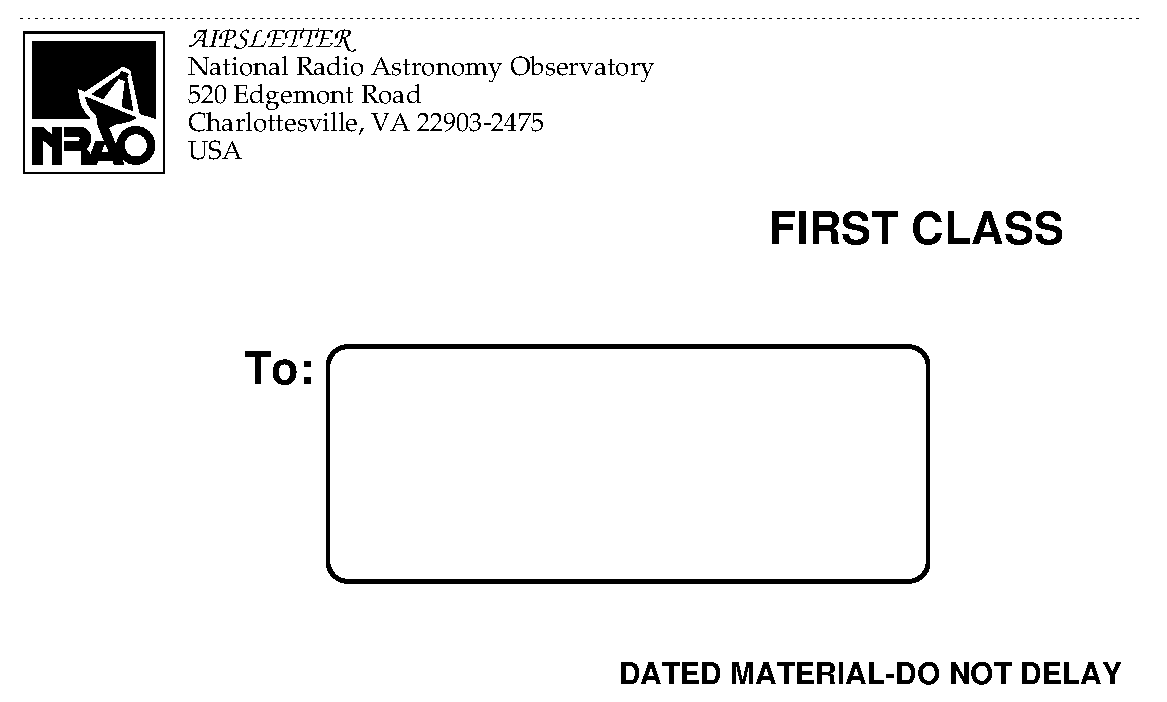
\includegraphics{FIG/AIPSLETM.PS}}}

\end{document}
